\documentclass[a4paper,12pt]{article}

\usepackage[utf8]{inputenc}
\usepackage{amsmath, amssymb}
\usepackage{graphicx}
\usepackage{booktabs}
\usepackage{siunitx}
\usepackage{caption}
\usepackage{subcaption}
\usepackage{geometry}
\usepackage{float}

\geometry{margin=2.5cm}

\graphicspath{{../graficos}{../graficos/planar_dielectric_waveguide}{../graficos/rectangular_dielectric_waveguide}}

\title{Análise de Resultados de Experimentos}
\author{Eduardo A. V. Souza, RA:250950}
\date{\today}

\begin{document}

\maketitle

\section{Semi-analytical analysis}
\label{sec:semi_analytical}

Let's begin the pre-analysis for solving the problem of a beam splitter by studiying some of the materials used in waveguides in the integrated circuit context. The dispersion relation for $Ag_3AsS_3$, $TiO_2$, $Si_3N_4$, and $SiO_2$ are equated in Eq. \ref{eq:disp_rel} and are shown in Fig. \ref{fig:ri_dispersion}. $Ag_3AsS_3$ is used in nonlinear optics: second-harmonic generation, $TiO_2$ is used in high-confinement waveguides in the visible and near-infrared spectrum, $Si_3N_4$ is used in nonlinear optics for supercontinuum generation, and $SiO_2$ is used in optical fibers and planar waveguides.

\begin{subequations}
    \begin{align}
        
    \end{align}
\end{subequations}

Figure \ref{fig:critical_angle} shows the critical angle as a function of the cladding refractive index for the core made of the materials stated above. You can see that as we increase the cladding RI (refractive index), the modes become more leaky and the critical angle increases, being easier to couple light in the waveguide. In the opposite direction, as we increase the core RI, the modes become more confined and the critical angle decreases, being harder to couple light in the waveguide.

\begin{figure}[H]
    \centering
    \begin{subfigure}{0.45\textwidth}
        \centering
        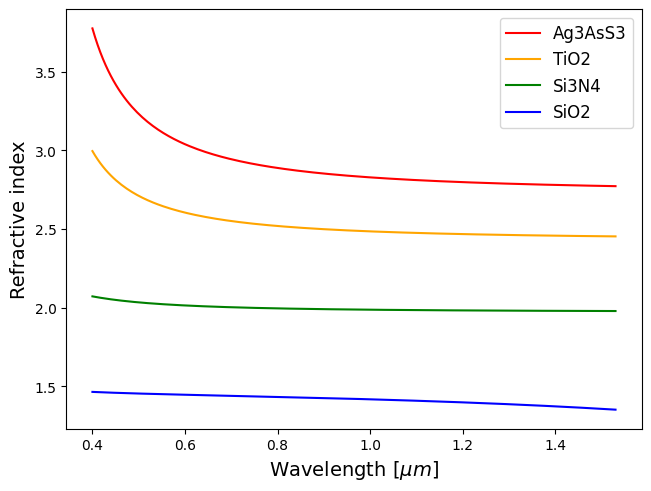
\includegraphics[scale=0.45]{dispersion_relation.png}
        \caption{Dispersion relation.}
        \label{fig:ri_dispersion}
    \end{subfigure}
    \hfill
    \begin{subfigure}{0.45\textwidth}
        \centering
        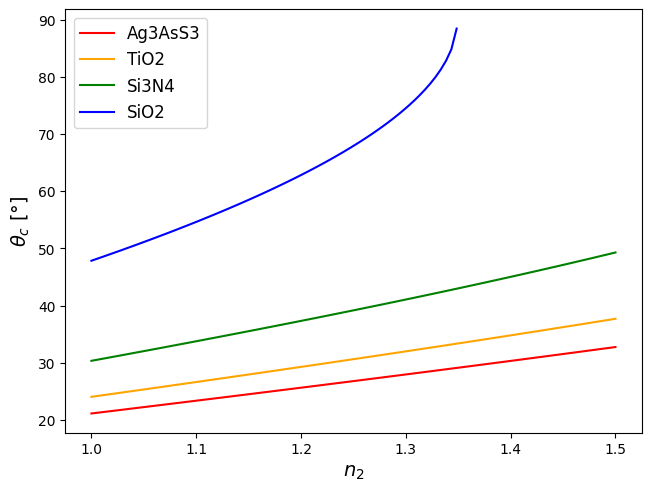
\includegraphics[scale=0.45]{critical_angle_vs_refractive_index.png}
        \caption{Critical angle.}
        \label{fig:critical_angle}
    \end{subfigure}
    \caption{Study of different materials for the core of the waveguide.}
\end{figure}

\subsection{Planar dielectric waveguide}
\label{subsec:planar_dielectric_waveguide}

A important parameter for waveguides is the numerical aperture ($NA$), which is a measure of the light acceptance angle in the waveguide. It is given by Eq. \ref{eq:NA}, where $n_1$ is the refractive index of the core and $n_2$ is the refractive index of the cladding. 

\begin{equation}
    NA = \sqrt{n_1^2 - n_2^2} 
    \label{eq:NA}
\end{equation}

The other important parameter is the critical angle ($\theta_c$), given by Eq. \ref{eq:theta_c}, related to the maximum angle of incidence for total internal reflection to occur.

\begin{equation}
    \theta_c = \sin^{-1} \left(\frac{n_2}{n_1}\right) 
    \label{eq:theta_c}
\end{equation}

The results for these parameters for $SiO_2$ and $TiO_2$ are shown in Tab. \ref{fig:na_theta_c}.

\begin{table}[H]
    \centering
    \begin{tabular}{ccc}
        \toprule
        Material & $\theta_c [^\circ]$ & $NA$ \\
        \midrule
        $SiO_2$ & 47.8 & 0.906 \\
        $TiO_2$ & 24.1 & 2.240 \\
        \bottomrule
    \end{tabular}
    \caption{Numerical aperture and critical angle for different core materials, considering air as the cladding.}
    \label{tab:na_theta_c}
\end{table}

A approximation for the number of TE modes is given by \eqref{eq:number_of_modes_approx}, where $d$ is the core thickness, $\lambda$ is the wavelength, and $NA$ is the numerical aperture. 

\begin{equation}
    M_{the} \doteq 2 \frac{d}{\lambda} NA
    \label{eq:number_of_modes_approx}
\end{equation}

The exact number of modes can be found by solving the characteristic equation for the planar dielectric waveguide, given by Eq. \ref{eq:char_eq}, where $m = 0, 1, 2, ...$ is the mode order, $k_0 = 2 \pi / \lambda$ is the free space wavenumber, $\theta_m$ is the angle of incidence for the m-th mode, and $\theta_c$ is the critical angle.

\begin{equation}
    f_1(\sin(\theta_m)) \equiv \tan\left[ \pi \left(\frac{\sin(\theta_m) d}{\lambda} - \frac{m}{2}\right) \right] =
    \sqrt{\frac{\sin^2(\overline{\theta}_c)}{\sin(\theta_m)^2} - 1}
    \label{eq:char_eq} \equiv f_2(\sin(\theta_m))
\end{equation}

The plot for $f_1$ and $f_2$ to help visualize the possible modes for the waveguide is shown in Fig. \ref{fig:char_eq}. Using the bisection or the Newton-Raphson methods based on the guess interval or point aided by Fig. \ref{fig:char_eq}, we can find the intersections of $f_1$ and $f_2$ to further calculate the propagation constant $\beta_m$ and the effective RI (ERI) $n_{eff,m}$ for the m-th order mode. The resultant modes are shown in Fig. \ref{fig:shell_modes} where the black dots are the modes, the green curve have radius $n_2 k_0$ and the blue curve have radius $n_2 k_0$. For a planal dielectric waveguide with $SiO_2$ as the core and with thickness $d = 10\mu$ we got 5 possible TE modes.

\begin{figure}[H]
    \centering
    \begin{subfigure}{0.45\textwidth}
        \centering
        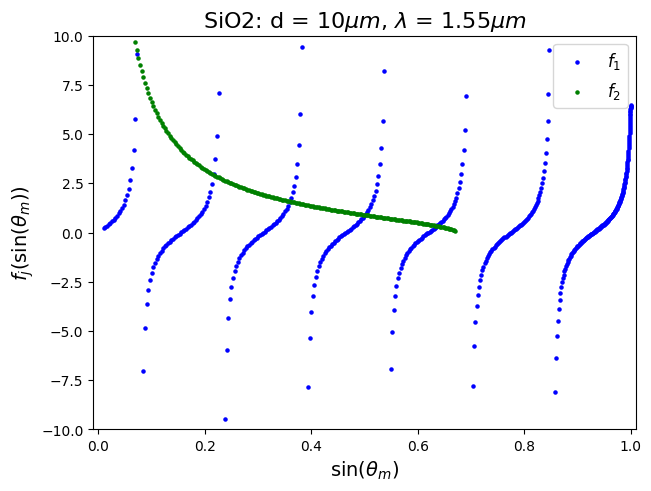
\includegraphics[scale=0.45]{modes_SiO2_d10um_wv1.55um.png}
        \caption{Characteristic equation.}
        \label{fig:char_eq}
    \end{subfigure}
    \hfill
    \begin{subfigure}{0.45\textwidth}
        \centering
        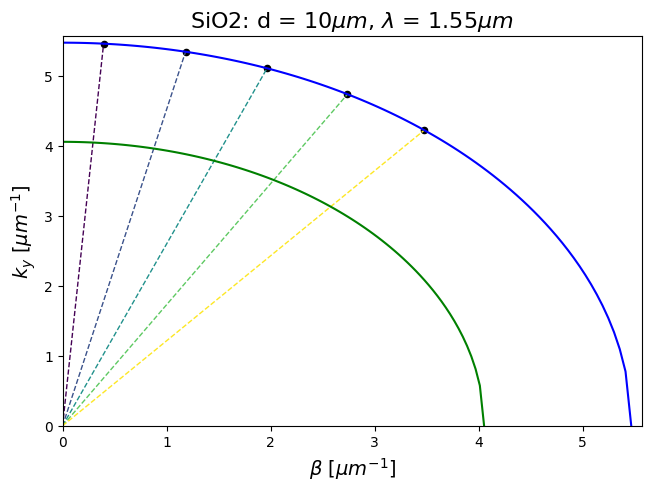
\includegraphics[scale=0.45]{modeshell_SiO2_d10um_wv1.55um.png}
        \caption{Guided modes.}
        \label{fig:shell_modes}
    \end{subfigure}
    \caption{Solution for the guided modes in a planar dielectric waveguide with a $SiO_2$ core, $d = 10 \mu m$ and $\lambda = 1.55 \mu m$.}
\end{figure}

A comparison between the approximation and exact number of TE modes is put in Tab. \ref{fig:number_of_modes_comparison} as we increase the thickness of the core, by consequence, we increase the number of possible modes. So, when it is possible to manually count the number of modes, use this technique to obtain the exact value, since the approximate value can diverge much.

\begin{table}[H]
    \centering
    \begin{tabular}{ccc}
        \toprule
        $d [\mu m]$ & $M_{app}$ & $M_{exa}$ \\
        \midrule
        1 & 2 & 1 \\
        5 & 6 & 3 \\
        10 & 12 & 5 \\
        \bottomrule
    \end{tabular}
    \caption{Approximate and exact number of TE modes for different core thicknesses for the $SiO_2$ waveguide.}
    \label{tab:number_of_modes_comparison}
\end{table}

Using the condition $k_0 n_2 \leq \beta_m \leq k_0 n_1$ to keep only the guided modes, we get the values for the propagation constant and the corresponding ERI for $SiO_2$-core waveguide in Tab. \ref{tab:beta_sio2}. Running the same simulation but for the $TiO_2$-core waveguide, we get the values of Tab. \ref{tab:beta_tio2}.

\begin{table}[H]
    \centering
    \begin{subtable}{0.45\textwidth}
        \centering
        \begin{tabular}{ccc}
            \toprule
            Mode & $\beta [\mu m^{-1}]$ & $n_{eff}$ \\
            \midrule
            0 & 5.419 & 1.337 \\
            1 & 5.008 & 1.235 \\
            2 & 4.171 & 1.029 \\
            \bottomrule
        \end{tabular}
        \caption{$SiO_2$.}
        \label{tab:beta_sio2}
    \end{subtable}
    \hfill
    \begin{subtable}{0.45\textwidth}
        \centering
        \begin{tabular}{ccc}
            \toprule
            Mode & $\beta [\mu m^{-1}]$ & $n_{eff}$ \\
            \midrule
            0 & 9.847 & 2.429 \\
            1 & 9.034 & 2.229 \\
            2 & 7.194 & 1.775 \\
            \bottomrule
        \end{tabular}
        \caption{$TiO_2$.}
        \label{tab:beta_tio2}
    \end{subtable}
    \caption{Propagation constant and effective refractive index in a planar dielectric waveguide with $d = 5 \mu m$ and $\lambda = 1.55 \mu m$.}
\end{table}

As we can see by the results above, the waveguide with core made by $TiO_2$ confines light much more than the one made by $SiO_2$. 

\subsection{Rectangular dielectric waveguide}
\label{subsec:rectangular_dielectric_waveguide}
    
Now, to solve the problem of a rectangular dielectric waveguide, we will use the Marcatili's approximation, that is, we will consider that $E(x, y) = X(x)Y(y)$. In other words, this problem is reduced to two planar dielectric waveguide problems (solved in Sec. \ref{subsec:planar_dielectric_waveguide}).

Let's start with the analysis of the number of modes for the waveguide made of $SiO_2$ with $w = 6\mu m$ and $t = 2\mu m$, for a input light with $\lambda = 1.55\mu m$. The characteristic equation and the diagram with the guided modes are shown in Fig. \ref{fig:char_eq2} and \ref{fig:shell_modes2}, respectively.

\begin{figure}[H]
    \centering
    \begin{subfigure}{0.45\textwidth}
        \centering
        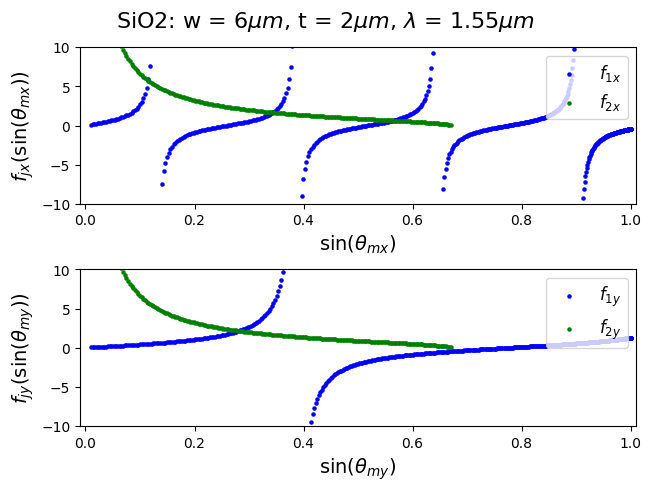
\includegraphics[scale=0.45]{modes_SiO2_w6um_t2um_wv1.55um.png}
        \caption{Characteristic equation.}
        \label{fig:char_eq2}
    \end{subfigure}
    \hfill
    \begin{subfigure}{0.45\textwidth}
        \centering
        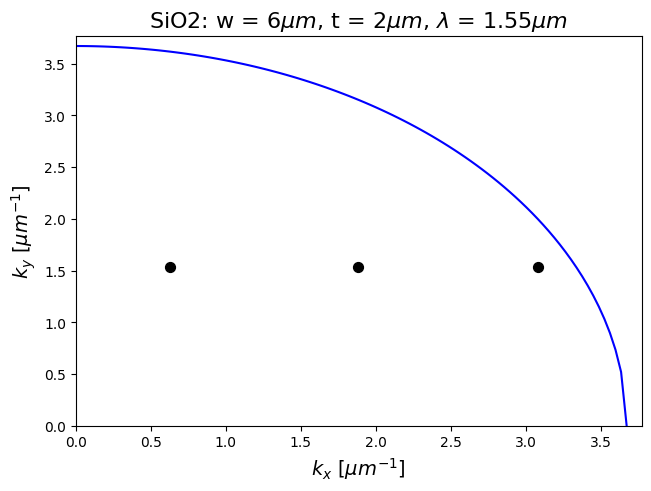
\includegraphics[scale=0.45]{modeshell_SiO2_w6um_t2um_wv1.55um.png}
        \caption{Guided modes.}
        \label{fig:shell_modes2}
    \end{subfigure}
    \caption{Solution for the guided modes in a rectangular dielectric waveguide with a $SiO_2$ core, $w = 6 \mu m$, $t = 2\mu m$, and $\lambda = 1.55 \mu m$.}
\end{figure}

The propagation constant and the refractive index for the guided modes are organized in Tab. \ref{tab:beta_sio2} for $SiO_2$ and in Tab. \ref{tab:beta_tio2} for $TiO_2$.

\begin{table}[H]
    \centering
    \begin{subtable}{0.45\textwidth}
        \centering
        \begin{tabular}{ccc}
            \toprule
            Mode & $\beta [\mu m^{-1}]$ & $n_{eff}$ \\
            \midrule
            (0,0) & 5.211 & 1.285 \\
            (1,0) & 4.901 & 1.209 \\
            (2,0) & 4.247 & 1.048 \\
            \bottomrule
        \end{tabular}
        \caption{$SiO_2$.}
    \end{subtable}
    \hfill
    \begin{subtable}{0.45\textwidth}
        \centering
        \begin{tabular}{ccc}
            \toprule
            Mode & $\beta [\mu m^{-1}]$ & $n_{eff}$ \\
            \midrule
            (0,0) & 9.401 & 2.319 \\
            (1,0) & 8.793 & 2.169 \\
            (2,0) & 7.453 & 1.839 \\
            (3,0) & 4.928 & 1.216 \\
            \bottomrule
        \end{tabular}
        \caption{$TiO_2$.}
        \label{tab:modes_d5um}
    \end{subtable}
    \caption{Propagation constant and effective refractive index in a rectangular dielectric waveguide with $w = 6 \mu m$, $t = 3\mu m$, and $\lambda = 1.55 \mu m$.}
\end{table}

As you can see by the results above, further from confining more the light inside the core, the $TiO_2$ waveguide also present one more mode than the $SiO_2$ waveguide for the same width and thickness parameters.

\section{COMSOL analysis}
\label{sec:comsol}

\subsection{Individual guides}
\label{subsec:individual_guides}

Now, let's model the rectangular dielectric waveguide in COMSOL Multiphysics and compare the results with those obtained using the Marcatili's method. Consider from now on the cladding material to be air ($n_2 = 1.000$), the input wavelength to be $\lambda = 1.55 \mu m$, the core width to be $w = 6 \mu m$ and the core thickness to be $t = 2 \mu m$.

Given the dispersion relation you can calculate the relative permittivity by Eq. \eqref{eq:eps_r}.

\begin{equation}
    \epsilon_r(\lambda) = \frac{n(\lambda)^2}{\mu_r(\lambda)}
    \label{eq:eps_r}
\end{equation}

Also, consider the following parameters for the first simulation:
\begin{itemize}
    \item Core material: $SiO_2$.
    \item Dispersion relation: Eq. \eqref{eq:sio2_func}.
    \item Relative permeability: 1.
\end{itemize}

Now consider the following parameters for the second simulation:
\begin{itemize}
    \item Core material: $TiO_2$.
    \item Dispersion relation: Eq. \eqref{eq:tio2_func}.
    \item Relative permeability: 1.
\end{itemize}

\subsection{Coupled guides}
\label{subsec:coupled_guides}

\end{document}